\newpage
\section{Introduction}
\label{sec:intro}

Network security has always been a warranted topic of concern in computer networks. A way to prevent or mitigate some of that concern on a network is to implement a firewall. Firewalls are able to prevent the spread of unwanted or malicious programs or data across networks/zones \parencite{blansit2009} and reduce the damage of a compromised network. While enterprise-level firewalls can cost upwards of \$40,000 USD \parencite{blueskysystems2025}, a local/home firewall can be made inexpensive using a Raspberry PI single-board computer (SBC) and open source software for significantly less \parencite{thepihut2025} \parencite{opnsense2025}. This project implements a lightweight firewall solution using a Raspberry Pi, turning the SBC into a dedicated network security device with multiple firewall zones and policies to ensure network traffic traverses the network as per the example in figure \ref{fig:basic-fw-diagram}. This will ensure proper packet filtering and traffic management on the network the firewall is used on.

\begin{figure}[H]
    \centering
    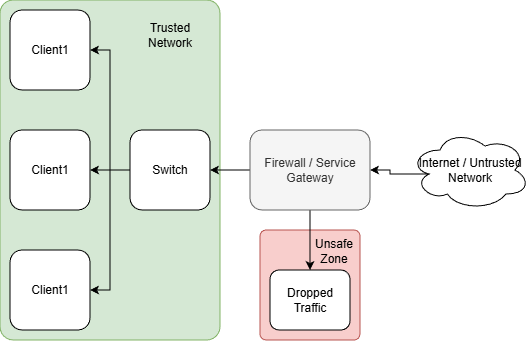
\includegraphics[width=0.6\linewidth]{Diagrams/os-fw-diagram.drawio.png}
    \caption{A diagram showcasing basic firewall filtering. showing how incoming traffic comes from the internet or an untrusted network, connects to the Firewall / Service gateway and is either passed to the LAN or dropped.}
    \label{fig:basic-fw-diagram}
\end{figure}

At its core, the coursework task put out is to install and configure a firewall application on a Raspberry Pi to act as a standalone firewall, as previously mentioned, while showing adequate knowledge and understanding of networking protocols (via traffic control, packet filtering, routing) and other approaches with self-hosting network devices, such as network monitoring and general observability \parencite{opencloudification2025} \parencite{dadiyala2023}. By using the Pi's onboard hardware and an additional network interface card (NIC), you can secure a home or small-to-medium-sized office network when paired with a Linux-based operating system like OPNsense \parencite{opnsense2025} (an open-source firewall and routing platform). OPNsense resembles a VM-based option for a service gateway (similar to Juniper's offering on its SRX line of hardware) that can provide routing, multi-WAN support, and VPNs, as well as firewall-specific features like network filtering, rule-based forwarding, and traffic (deep packet) inspection. What makes it more than just a firewall (a service gateway) is that it operates at all layers of the OSI model, not just layers 1-4. This project creates a general network service gateway capable of managing traffic between three distinct network interfaces, each representing different security zones.

\begin{figure}[H]
    \centering
    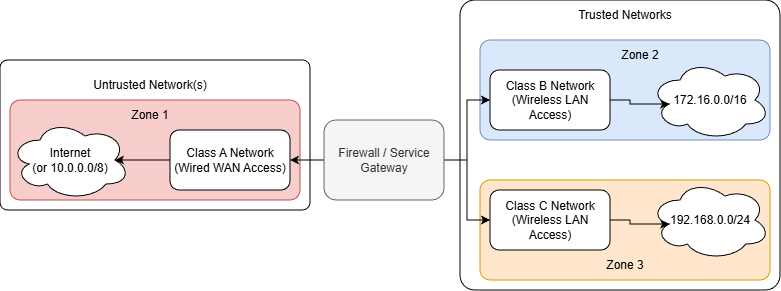
\includegraphics[width=0.8\linewidth]{Diagrams/os-fw-implementation-diagram.drawio.png}
    \caption{A diagram showing the different network ranges, the interfaces (and types) they're connected to and how they'll be isolated and sat within different firewall zones.}
    \label{fig:basic-fw-breakdown}
\end{figure}

TO EXPLAIN DIFFERENCES BETWEEN CLASSFUL NETWORK DECLARATIONS

This task calls for building a multi-interface firewall supporting Class-A, Class-B, and Class-C networks (as highlighted in Figure \ref{fig:basic-fw-breakdown}), and implementing firewall policies including default-deny rules and essential service permissions (allowing DNS, DHCP, and ICMP traffic) between the zones. Moreover, the work should allow internal/management network communication (to access the firewall), network address translation for internet access, and some form of logging for analysis and troubleshooting. Furthermore, the project calls for performance monitoring and evaluation to assess the system’s scalability and effectiveness under various traffic conditions outlined in the brief.